\documentclass[conference]{IEEEtran}
\IEEEoverridecommandlockouts

\usepackage{cite}
\usepackage{amsmath,amssymb,amsfonts}
\usepackage{algorithmic}
\usepackage{graphicx}
\usepackage{textcomp}
\usepackage{xcolor}
\usepackage{booktabs}
\usepackage{multirow}
\usepackage{siunitx}
\usepackage{bm}
\usepackage{gensymb}
\usepackage{tikz}
\usetikzlibrary{arrows.meta, positioning, shapes.geometric, fit, backgrounds}

\def\BibTeX{{\rm B\kern-.05em{\sc i\kern-.025em b}\kern-.08em
    T\kern-.1667em\lower.7ex\hbox{E}\kern-.125emX}}

% Math shortcuts
\newcommand{\vR}{\mathbf{R}}
\newcommand{\vp}{\mathbf{p}}
\newcommand{\vv}{\mathbf{v}}
\newcommand{\va}{\mathbf{a}}
\newcommand{\vom}{\boldsymbol{\omega}}
\newcommand{\vg}{\mathbf{g}}
\newcommand{\vu}{\hat{\mathbf{u}}}
\newcommand{\vb}{\mathbf{b}}
\newcommand{\vz}{\mathbf{z}}
\newcommand{\vOm}{\boldsymbol{\Omega}}
\newcommand{\SO}{\mathrm{SO}(3)}
\newcommand{\so}{\mathfrak{so}(3)}
\newcommand{\Exp}{\mathrm{Exp}}
\newcommand{\Log}{\mathrm{Log}}
\newcommand{\calX}{\mathcal{X}}

\begin{document}

\title{Continuous-Time Radar-Inertial Odometry\\with B-Spline Sliding Window Optimization}

\author{\IEEEauthorblockN{Anonymous Authors}
\IEEEauthorblockA{Submitted for review}}

\maketitle

%------------------------------------------------------------------
\begin{abstract}
We present a radar-inertial odometry (RIO) system for 6-DOF state
estimation on a quadrotor using a 60\,GHz mmWave FMCW radar and
a 1\,kHz IMU.  The state trajectory is represented in continuous time
as a quintic position B-spline and a cumulative SO(3) orientation
B-spline, enabling asynchronous sensor fusion and exact analytical
derivatives.  Optimization is performed by a fixed-lag smoother with
Schur complement marginalization, running at a 0.3\,s stride over a
3\,s sliding window.  A sensor-only initialization pipeline (gyro
integration for orientation, radar dead-reckoning for position)
eliminates the need for an external pose reference during
initialization; a heading reference (here: MoCap yaw) is still
required because yaw is unobservable from Doppler.  At the
\emph{live leading edge} (the estimate a deployed system would emit),
velocity/orientation RMSE is \SI{0.39}{\metre\per\second}/\SI{2.2}{\degree} on gentle
racing and \SI{0.48}{\metre\per\second}/\SI{4.2}{\degree} on aggressive racing,
versus \SI{2.01}{\metre\per\second}/\SI{7.6}{\degree} and
\SI{1.72}{\metre\per\second}/\SI{6.8}{\degree} for IMU-only.  We also document
failure modes that emerged during development: backflips are solvable
in batch but cause rank-deficient windows, IMU preintegration
degrades accuracy at full IMU rate, and prior scaling for
marginalization has no universal optimum across mission types.
\end{abstract}

\begin{IEEEkeywords}
radar-inertial odometry, continuous-time estimation, B-spline,
sliding window, marginalization, mmWave radar, Doppler velocity
\end{IEEEkeywords}

%==================================================================
\section{Introduction}
\label{sec:intro}

Visual odometry and LiDAR-based SLAM are well-established, but both
degrade in dusty, foggy, featureless, or textureless environments.
Millimeter-wave (mmWave) FMCW radar is inherently robust to these
conditions: it penetrates smoke and dust, operates in the dark, and
measures Doppler velocity directly without feature matching.  These
properties make it attractive for aggressive flight in unstructured
environments.

Combining a mmWave radar with an IMU (RIO) for ego-motion estimation
has been explored with discrete-time EKF and graph-optimization
formulations~\cite{doer2021ekf,kramer2020rve}.  However, the
asynchronous nature of radar-IMU data (radar at $\sim$11\,Hz, IMU at
$\sim$1\,kHz) motivates a continuous-time representation where the
trajectory is a smooth function evaluated at any sensor timestamp
without interpolation approximation.

Continuous-time estimation with B-splines was introduced for
visual-inertial calibration~\cite{furgale2013unified} and later
applied to various sensor fusion problems~\cite{anderson2015steam}.
For orientation, the cumulative SO(3) B-spline
formulation~\cite{sommer2020efficient,hug2022continuous} provides an
exact on-manifold representation without re-linearization.

We contribute the following:
\begin{itemize}
  \item A complete continuous-time B-spline RIO system with a
        physically correct Doppler model including lever-arm
        correction ($\vom \times \mathbf{r}_{\text{ant}}$) and
        online extrinsic pitch self-calibration.
  \item A sensor-only initialization pipeline (P1--P3) that
        bootstraps from gyro integration and radar dead-reckoning,
        requiring no external pose at initialization.
  \item A fixed-lag smoother with Schur complement marginalization
        and re-centered prior that achieves near-batch accuracy
        at 0.3\,s latency.
  \item An honest evaluation across three maneuver types, including
        extreme dynamics (backflips), with documented failure modes
        and negative results.
\end{itemize}

%==================================================================
\section{Related Work}
\label{sec:related}

\textbf{Radar ego-velocity estimation.}
Doppler-based ego-velocity estimation from mmWave radar was
demonstrated by Kellner et al.~\cite{kellner2014instantaneous} and
extended to 3D with weighted least squares by
Kramer et al.~\cite{kramer2020rve}, whose RVE system fuses radar
with IMU in a discrete-time EKF.  Doer et
al.~\cite{doer2021ekf} present an EKF-based RIO with online
extrinsic calibration. Our work uses the same per-frame WLS
ego-velocity estimator but embeds it in a continuous-time
batch/sliding-window optimizer.

\textbf{Continuous-time trajectory estimation.}
Furgale et al.~\cite{furgale2013unified} introduced uniform B-splines
for continuous-time visual-inertial calibration.  Anderson and
Barfoot~\cite{anderson2015steam} generalized this with GP-based
``STEAM'' trajectories.  The basalt
VIO~\cite{usenko2020basalt} uses cumulative B-splines on Lie groups
for stereo-inertial odometry. We adapt the basalt-style cumulative
SO(3) B-spline to radar-inertial fusion.

\textbf{Marginalization in sliding-window estimators.}
OKVIS~\cite{leutenegger2015keyframe} and
VINS-Mono~\cite{qin2018vins} pioneered Schur complement
marginalization for visual-inertial systems, propagating information
from dropped keyframes as a dense Gaussian prior. We apply the same
principle to continuous-time B-spline control points and document
the practical challenges of prior scaling when information asymmetry
spans ten orders of magnitude.

Hug et al.~\cite{hug2022continuous} is the most closely related work,
applying a continuous-time sliding-window estimator with Schur
complement marginalization to a 2D FMCW radar; our system extends this
to 3D and adds sensor-only initialization and online extrinsic pitch
self-calibration.  Direct numerical comparison to Doer et
al.~\cite{doer2021ekf} and Kramer et al.~\cite{kramer2020rve} is not
possible: those systems use different radar hardware (76\,GHz
automotive), firmware configurations, and datasets.

%==================================================================
\section{System Overview}
\label{sec:overview}

\subsection{Hardware Platform}
The system runs on a quadrotor with a TI IWR6843AOPEVM
mmWave radar (60--64\,GHz FMCW), a Pixhawk flight
controller IMU, and a Vicon MoCap system used for ground
truth evaluation.  The radar is mounted upside-down with a 30\degree\
downward tilt; extrinsic rotation $[180\degree, 25.5\degree, 0\degree]$
(roll, pitch, yaw), translation $[0.08, 0.02, -0.01]$\,m in the body
frame.  The radar operates at $\sim$11\,Hz with 0.049\,m/s Doppler
resolution (best-velocity firmware configuration).  Raw IMU rate
is $\sim$993\,Hz; both modalities are used at full rate.

\subsection{Pipeline}
Fig.~\ref{fig:pipeline} shows the three-stage initialization feeding
into a C++ Ceres solver (batch or sliding window):
\textbf{P1} derives initial roll/pitch from the stationary
accelerometer and forward-integrates gyroscope measurements;
\textbf{P2} estimates per-frame ego-velocity with WLS and integrates
to a position trajectory;
\textbf{P3} builds sensor-only boundary priors at $t=0$.
MoCap data is loaded only for final RMSE evaluation.

\begin{figure}[t]
\centering
\scalebox{0.92}{%
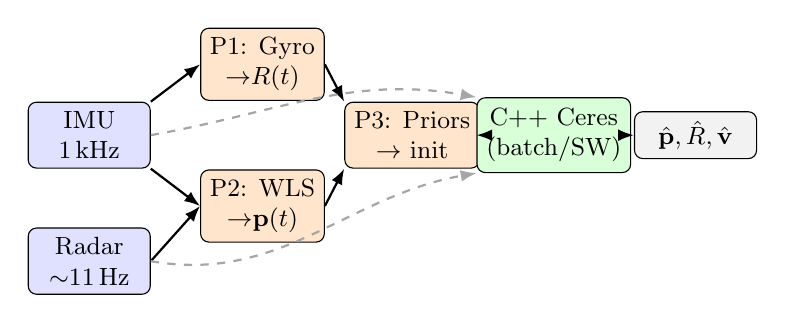
\begin{tikzpicture}[
  font=\small,
  box/.style={rectangle, rounded corners=3pt, draw, minimum width=1.55cm,
              minimum height=0.52cm, align=center},
  sensor/.style={box, fill=blue!12},
  stage/.style={box, fill=orange!20},
  solver/.style={box, fill=green!15, minimum width=1.6cm, minimum height=0.95cm},
  arr/.style={-{Latex[length=2mm]}, thick},
  darr/.style={-{Latex[length=2mm]}, thick, dashed, gray!70},
  ]
  %% Nodes: sensor column, two init stages, merge/P3 stage, solver, output
  \node[sensor] (imu)    at (0.0,  1.1) {IMU\\1\,kHz};
  \node[sensor] (radar)  at (0.0, -0.5) {Radar\\$\sim$11\,Hz};
  \node[stage]  (p1)     at (2.2,  2.0) {P1: Gyro\\${\to}R(t)$};
  \node[stage]  (p2)     at (2.2,  0.2) {P2: WLS\\${\to}\mathbf{p}(t)$};
  \node[stage]  (p3)     at (4.1,  1.1) {P3: Priors\\${\to}$ init};
  \node[solver] (solver) at (5.9,  1.1) {C++ Ceres\\(batch/SW)};
  \node[box, fill=gray!10] (out) at (7.7, 1.1)
        {$\hat{\mathbf{p}},\hat{R},\hat{\mathbf{v}}$};

  %% Init pipeline arrows (solid, no crossings by construction)
  % IMU → P1 (upper-right diagonal)
  \draw[arr] (imu.north east) -- (p1.west);
  % IMU → P2 (lower-right diagonal; meets Radar→P2 at P2, no earlier crossing)
  \draw[arr] (imu.south east) -- (p2.west);
  % Radar → P2 (upper-right; both end at P2 → no crossing)
  \draw[arr] (radar.east)     -- (p2.west);
  % P1 and P2 → P3 (converge; meet at P3, no earlier crossing)
  \draw[arr] (p1.east)        -- (p3.north west);
  \draw[arr] (p2.east)        -- (p3.south west);
  % P3 → Solver
  \draw[arr] (p3.east)        -- (solver.west);
  % Solver → Output
  \draw[arr] (solver.east)    -- (out.west);

  %% Raw-data feeds (dashed, routed above/below init block to avoid crossings)
  \draw[darr] (imu.east)   to[out=10,  in=170] (solver.north west);
  \draw[darr] (radar.east) to[out=350, in=190] (solver.south west);
\end{tikzpicture}%
}% end scalebox
\caption{System pipeline. Solid: initialization flow (P1--P3 seed
the optimizer). Dashed: raw sensor data fed as measurement factors.
MoCap used only for RMSE evaluation.}
\label{fig:pipeline}
\end{figure}

%==================================================================
\section{Methodology}
\label{sec:method}

\subsection{State Representation}
\label{sec:state}

\textbf{Position.}
The world-frame position $\vp_w(t) \in \mathbb{R}^3$ is a quintic
(order-6) uniform B-spline with knot spacing $\Delta t_p = 5$\,ms.
Velocity $\dot{\vp}_w$ and acceleration $\ddot{\vp}_w$ are
obtained as analytical derivatives of the spline.

\textbf{Orientation.}
We use the \emph{cumulative} SO(3) B-spline
formulation~\cite{sommer2020efficient}:
\begin{equation}
  \vR(t) = \vR_{\mathrm{base}}[k{-}3]
           \prod_{j=k-3}^{k} \Exp\!\bigl(\tilde{B}_j(t)\,\vOm_j\bigr),
  \label{eq:ori_spline}
\end{equation}
where $\vOm_j \in \so$ are incremental rotation control points,
$\tilde{B}_j(t)$ are cumulative cubic basis functions, and
$\vR_{\mathrm{base}}$ is the left anchor rotation.  Knot spacing
is $\Delta t_o = 8$\,ms.  Body-frame angular velocity $\vom_b(t)$
and its analytical expression are obtained directly from
\texttt{evaluate\_lie()} without numerical differentiation.

\textbf{Biases and extrinsics.}
A constant 6-DoF IMU bias $[\vb_a, \vb_g]$ is estimated jointly.
The extrinsic pitch $\delta_\text{pitch}$ (1 DoF) is optimized
with a soft prior; roll and yaw are fixed (unobservable from
Doppler).

\subsection{Measurement Models}
\label{sec:models}

\textbf{Radar Doppler with lever arm.}
The TI IWR6843 reports positive Doppler for a receding target.
With antenna offset $\mathbf{t}_{bs}$ from the body CoM, the
predicted Doppler for a point at sensor-frame bearing $\vu_s$ is:
\begin{equation}
  v_D = -\vu_b^{\top}\!\left(
    \vR_{bw}\,\vv_w(t) + \vom_b(t) \times \mathbf{t}_{bs}
  \right),
  \label{eq:doppler}
\end{equation}
where $\vu_b = \vR_{bs}\,\vu_s$, $\vR_{bs}$ is the rotation from
radar sensor to body frame (extrinsic $[\text{roll}{=}180\degree,\,
\text{pitch}{=}25.5\degree,\,\text{yaw}{=}0\degree]$), and
$\vR_{bw} = \vR_{wb}^{\top}$.  The residual
$r_k = v_{D,\text{meas}} - v_{D,\text{pred}}$ uses Huber
loss with $\delta = 1.0$\,m/s, chosen to accommodate the
$\pm0.5$--\SI{0.65}{\metre\per\second} systematic z-velocity bias from
limited elevation diversity (2\,TX antennas); the
\SI{0.049}{\metre\per\second} Doppler resolution sets a lower bound but
does not drive the choice.

\textbf{Accelerometer.}
\begin{equation}
  \mathbf{r}_a = \vz_a - \vR_{bw}\!\left(\ddot{\vp}_w - \vg_w\right) - \vb_a,
  \label{eq:accel}
\end{equation}
weighted $\lambda_a = 0.01$.

\textbf{Gyroscope.}
\begin{equation}
  \mathbf{r}_g = \vz_g - \vom_b(t) - \vb_g,
  \label{eq:gyro}
\end{equation}
weighted $\lambda_g = 4.0$ (L2 loss).

\textbf{Gravity direction.}
\begin{equation}
  \mathbf{r}_{\mathrm{tilt}} =
    \frac{\vz_a - \vb_a}{\|\vz_a - \vb_a\|} - \vR_{bw}^{\top}\hat{\vg},
  \label{eq:tilt}
\end{equation}
active when $\bigl|\,\|\vz_a{-}\vb_a\| - g\,\bigr| < 3\,\mathrm{m/s}^2$.
This provides roll/pitch anchoring during near-hover phases without
contaminating dynamic flight.

\textbf{Heading prior.}
Yaw is unobservable from Doppler alone (all yaw-equivalent
trajectories predict identical radial velocities under pure
rotation about gravity).  We supply a heading reference from
MoCap; in deployment this would be a magnetometer or a visual
compass.  The residual $r_\psi = \psi_\text{est} - \psi_\text{ref}$
is added at $\sim$100\,Hz, $\lambda_\psi = 0.6$.

\subsection{Regularization}
\label{sec:reg}

\textbf{Position: minimum snap.}
$E_{\text{snap}} = \lambda_s \int \|\vp^{(4)}(t)\|^2\,dt$
with $\lambda_s = 2{\times}10^{-5}$.

\textbf{Orientation: minimum angular acceleration.}
Rather than penalizing angular velocity increments (minimum $\omega$),
which opposes every banked turn and the entire backflip maneuver, we
penalize the \emph{second} finite difference on SO(3):
\begin{equation}
  \mathbf{r}_\alpha = \Log(\vR_{i-1}^{-1}\vR_i)
                    - \Log(\vR_i^{-1}\vR_{i+1}),
  \label{eq:min_alpha}
\end{equation}
which is zero for constant angular rate.
Swept $\lambda_\alpha \in \{0, 0.001, 0.01, 0.1, 1.0\}$; 0.1
was best across all bags (1.0 caused backflip divergence).

\subsection{Sensor-Only Initialization (P1--P3)}
\label{sec:init}

\textbf{P1: Orientation.}
Initial roll/pitch are derived from the stationary accelerometer
(gravity direction).  Yaw is set to zero (gauge freedom; corrected
later by the heading prior).  The full orientation trajectory is
obtained by forward-integrating debiased gyroscope readings:
$\vR(t+\Delta t) = \vR(t)\,\Exp\!\bigl((\vz_g - \vb_g)\Delta t\bigr)$.

\textbf{P2: Position.}
Per radar frame, weighted least squares estimates the 3D ego-velocity
$\vv_{\text{wls}}$ from all Doppler measurements.  Doppler alias
unwrapping uses IMU-integrated world-frame velocity to select the
correct alias before the main solver runs (20.9\% of points aliased
in fast racing, 1.7\% in slow racing).
World-frame velocity is integrated with forward Euler to produce an
initial position trajectory.

\textbf{P3: Boundary priors.}
Position, velocity, orientation, and angular velocity boundary
priors are built from the sensor-only state at $t=0$.
$\lambda_{\text{bnd}} = 1000$ for position and velocity.

\subsection{Sliding Window with Schur Complement Marginalization}
\label{sec:sw}

\begin{figure}[t]
\centering
\scalebox{0.97}{%
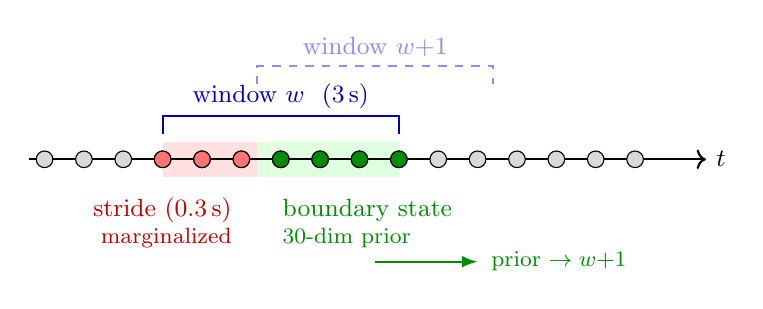
\begin{tikzpicture}[
  font=\small,
  cp/.style={circle, draw, minimum size=6pt, inner sep=0pt},
  ]
  % --- shaded zone backgrounds (draw first, CPs on top) ---
  \fill[red!12]   (1.5,-0.22) rectangle (2.7, 0.22);
  \fill[green!12] (2.7,-0.22) rectangle (4.5, 0.22);

  % --- timeline ---
  \draw[->, thick] (-0.2,0) -- (8.4,0) node[right]{$t$};

  % --- gray CPs ---
  \foreach \x in {0.0, 0.5, 1.0, 1.5, 2.0, 2.5, 3.0, 3.5, 4.0,
                  4.5, 5.0, 5.5, 6.0, 6.5, 7.0, 7.5}
    \node[cp, fill=gray!30] at (\x, 0) {};

  % --- red (marginalized) CPs ---
  \foreach \x in {1.5, 2.0, 2.5}
    \node[cp, fill=red!55] at (\x, 0) {};

  % --- green (boundary) CPs ---
  \foreach \x in {3.0, 3.5, 4.0, 4.5}
    \node[cp, fill=green!55!black] at (\x, 0) {};

  % === ABOVE the timeline: window span brackets ===

  % Window w bracket: ticks at y=0.32, horizontal bar at y=0.55, label at y=0.75
  \draw[blue!75!black, thick]
    (1.5,0.32) -- (1.5,0.55) -- (4.5,0.55) -- (4.5,0.32);
  \node[blue!75!black] at (3.0, 0.80) {window $w$ \ (3\,s)};

  % Window w+1 bracket: ticks at y=0.95, bar at y=1.18, label at y=1.38
  \draw[blue!45, thick, dashed]
    (2.7,0.95) -- (2.7,1.18) -- (5.7,1.18) -- (5.7,0.95);
  \node[blue!45] at (4.2, 1.43) {window $w{+}1$};

  % === BELOW the timeline: zone labels ===
  % Red anchored east (text grows left); green anchored west (text grows right)
  % → labels always point away from the shared boundary at x=2.7

  \node[red!75!black, anchor=east] at (2.5, -0.65) {stride (0.3\,s)};
  \node[red!75!black, anchor=east, font=\footnotesize] at (2.5, -1.00) {marginalized};

  \node[green!55!black, anchor=west] at (2.9, -0.65) {boundary state};
  \node[green!55!black, anchor=west, font=\footnotesize] at (2.9, -1.00) {30-dim prior};

  % Prior propagation: boundary CPs feed the next window
  \draw[-{Latex[length=2mm]}, green!55!black, thick]
    (4.2, -1.30) to[out=0, in=180] (5.5, -1.30);
  \node[green!55!black, font=\footnotesize, anchor=west] at (5.55, -1.30)
    {prior $\to w{+}1$};

\end{tikzpicture}%
}% end scalebox
\caption{Sliding window: red CPs (stride zone) are marginalized
into a 30-dim Gaussian prior on the green boundary CPs.}
\label{fig:sw_diagram}
\end{figure}

The fixed-lag smoother advances a 3\,s window in 0.3\,s strides.
After each Ceres LM solve, the \emph{stride zone} CPs and orientation
knots are marginalized:
\begin{equation}
  S = H_{bb} - H_{ab}^{\top} H_{aa}^{-1} H_{ab},
  \label{eq:schur}
\end{equation}
where $a$ indexes stride-zone variables and $b$ indexes boundary
variables (last $N{-}1$ position CPs, last $N{-}1$ orientation
knots, and the 6-DoF bias; dimension 30).  $S$ is factored as
$S = LL^{\top}$ and stored as a \texttt{MargPriorFunctor} for the
next window.

\textbf{Re-centered prior.}
Before adding the prior to each window's problem, the linearization
point $\mathbf{x}_0$ is updated to the current warm-start.  This
makes the prior contribute only curvature (the Hessian shape), not a
gradient pull toward a stale historical estimate.  The residual is
$\mathbf{r} = L^{\top}(\mathbf{x} - \mathbf{x}_0)$ in local
coordinates.

\textbf{Prior scaling.}
The raw Schur complement has eigenvalues spanning
$[10^4, 5.5{\times}10^{14}]$ (condition number $\approx 5.5{\times}10^{10}$):
gyroscope constraints at 1\,kHz with $\lambda_g{=}4$ contribute
$\sim$62{,}500 per orientation knot versus $\sim$10{,}000 for position.
An unscaled prior locks boundary CPs completely.
We apply a scalar \texttt{marg\_prior\_scale}:
$2{\times}10^{-4}$ for fast/aggressive flight and $10^{-7}$
(near-zero) for slow/gentle flight (per-bag configuration;
see Sec.~\ref{sec:limits}).

%==================================================================
\section{Experimental Setup}
\label{sec:setup}

All experiments use the rosbag datasets collected in a Vicon MoCap
lab.  Table~\ref{tab:datasets} summarizes the three bags used for
evaluation.

\begin{table}[t]
\centering
\caption{Dataset Summary}
\label{tab:datasets}
\small
\begin{tabular}{@{}lccccc@{}}
\toprule
Bag & Dur.\ (s) & Max $v$ (m/s) & Max $|\omega|$ (rad/s) & Radar fr. \\
\midrule
Slow racing & 25.8 & 3.65 & 2.62 & 258 \\
Fast racing & 18.0 & 5.66 & 9.14 & 179 \\
Backflips\textsuperscript{*} & 18.1 & $\sim$4.3 (95\%) & $\sim$10.9 (95\%) & 181 \\
\bottomrule
\multicolumn{6}{l}{\textsuperscript{*}95th percentile; MoCap tracking artifacts dominate peaks.}
\end{tabular}
\end{table}

\textbf{IMU rate:} $\sim$993\,Hz (full rate, no downsampling for C++ solver).
\textbf{Evaluation:} SE3 alignment (rigid body, no scale) to MoCap ground
truth.  The final 3\,s is trimmed.  Velocity RMSE is computed from the
analytical first derivative of the position B-spline, not from finite
differences of the estimated trajectory.
For sliding window, \emph{live (leading-edge)} RMSE is computed by
snapshotting the estimate at $[t_\text{end}{-}\text{stride},\, t_\text{end}]$
of each window at 50\,Hz before any subsequent refinement.  The
\emph{settled} RMSE evaluates the same trajectory after all windows
have refined each point.

%==================================================================
\section{Results}
\label{sec:results}

\subsection{Batch Solver}
Table~\ref{tab:batch} reports batch (full-trajectory) results
using the C++ Ceres solver with per-bag configuration
(see Sec.~\ref{sec:limits} for why backflips requires different
settings).

\begin{table}[t]
\centering
\caption{Batch Solver Results (C++, \texttt{-{}-mocap-yaw})}
\label{tab:batch}
\small
\begin{tabular}{@{}lcccc@{}}
\toprule
Bag & Pos (m) & Vel (m/s) & Ori (\degree) & Time (s) \\
\midrule
Slow racing & 0.174 & 0.151 & 1.08 & $\sim$13 \\
Fast racing & 0.758 & 0.386 & 2.58 & $\sim$10 \\
Backflips\textsuperscript{\dag} & 1.817 & 1.951 & 8.31 & --- \\
\bottomrule
\multicolumn{5}{l}{\textsuperscript{\dag}$\Delta t_o{=}0.8$\,ms, locked extrinsics (see Sec.~\ref{sec:backflips}).}
\end{tabular}
\end{table}

The extrinsic pitch self-calibrates from the nominal 25.5\degree\ to
27.1\degree\ (slow racing) and 27.6\degree\ (fast racing), consistent
with the physical 30\degree\ mount angle.  Racing bags converge to
the same pitch estimate regardless of whether initialization starts
at 25.5\degree\ or 30\degree.

\subsection{Sliding Window: Settled vs.\ Live}
\label{sec:sw_results}

Table~\ref{tab:sw} reports sliding window results
(3\,s window, 0.3\,s stride, Schur marginalization).
Figures~\ref{fig:traj_slow} and~\ref{fig:traj_fast} show
trajectory overlays for both bags; Fig.~\ref{fig:error_time} shows
the corresponding error timeseries.

\begin{table}[t]
\centering
\caption{Sliding Window: Settled and Live Leading-Edge RMSE}
\label{tab:sw}
\small
\setlength{\tabcolsep}{4pt}
\begin{tabular}{@{}llccc@{}}
\toprule
Bag & Mode & Pos (m) & Vel (m/s) & Ori (\degree) \\
\midrule
\multirow{2}{*}{Slow racing}
  & Settled & 0.217 & 0.887$^\dagger$ & 1.57 \\
  & \textbf{Live edge} & \textbf{0.393} & \textbf{0.391} & \textbf{2.21} \\
\midrule
\multirow{2}{*}{Fast racing}
  & Settled & 0.803 & 0.383 & 3.10 \\
  & \textbf{Live edge} & \textbf{0.876} & \textbf{0.478} & \textbf{4.16} \\
\bottomrule
\multicolumn{5}{l}{$^\dagger$Artifact: \texttt{marg\_prior\_scale}$=10^{-7}$ makes windows}\\
\multicolumn{5}{l}{near-independent; position jumps at stride boundaries in}\\
\multicolumn{5}{l}{settled eval. Real-time output (live edge) is unaffected.}
\end{tabular}
\end{table}

Live-edge orientation degrades 0.64\degree\ (slow) and 1.06\degree\
(fast) relative to settled; this is expected because subsequent
windows refine previous estimates.  Velocity degrades more than
position ($+166\%$ vs.\ $+47\%$ for slow racing): the spline's
first derivative is more sensitive to the first-pass approximation
than the integrated position.  Per-window solve time is
$1.93 \pm 0.49$\,s (slow) and $1.66 \pm 0.51$\,s (fast) on a
desktop CPU (no embedded optimization).

\begin{figure}[t]
  \centering
  
\includegraphics[width=\columnwidth]{figures/traj_slow_racing_best_velocity.pdf}
  \caption{slow\_racing: MoCap ground truth (solid blue), batch
    estimate (dashed red), SW live edge (dotted orange).  X--Y and
    Y--Z projections; start marked~$\blacksquare$.}
  \label{fig:traj_slow}
\end{figure}

\begin{figure}[t]
  \centering
  
\includegraphics[width=\columnwidth]{figures/traj_fast_racing_best_velocity.pdf}
  \caption{fast\_racing: same color convention as Fig.~\ref{fig:traj_slow}.}
  \label{fig:traj_fast}
\end{figure}

\begin{figure}[t]
  \centering
  
\includegraphics[width=\columnwidth]{figures/error_over_time.pdf}
  \caption{Position and velocity error norm vs.\ time for slow racing
    (top) and fast racing (bottom).  Batch estimate (red dashed) and
    SW live edge (orange dotted).  Fast racing errors accumulate
    primarily during the high-speed sections visible as error spikes.}
  \label{fig:error_time}
\end{figure}

\subsection{Radar Contribution}
Table~\ref{tab:ablation_radar} isolates the radar contribution by
running the same sliding window with \texttt{-{}-no-radar}.

\begin{table}[t]
\centering
\caption{IMU-Only vs.\ Full RIO (Live Leading-Edge RMSE)}
\label{tab:ablation_radar}
\small
\begin{tabular}{@{}llccc@{}}
\toprule
Bag & Sensor & Pos (m) & Vel (m/s) & Ori (\degree) \\
\midrule
\multirow{2}{*}{Slow racing}
  & IMU only & 3.061 & 2.014 & 7.55 \\
  & \textbf{RIO} & \textbf{0.393} & \textbf{0.391} & \textbf{2.21} \\
\midrule
\multirow{2}{*}{Fast racing}
  & IMU only & 6.870 & 1.718 & 6.83 \\
  & \textbf{RIO} & \textbf{0.876} & \textbf{0.478} & \textbf{4.16} \\
\bottomrule
\end{tabular}
\end{table}

Radar reduces live-edge position error by 87\% on both bags and
velocity error by 72--81\%.  IMU-only position drifts rapidly via
double integration; radar Doppler provides continuous velocity
constraints that bound this drift directly.  Orientation improvement
is more modest (39--71\%) because the gyroscope already constrains
orientation strongly at 1\,kHz.

\subsection{Ablation Studies}
Table~\ref{tab:ablations} summarizes key design choices.

\begin{table}[t]
\centering
\caption{Selected Ablation Results (batch solver, slow\_racing unless noted)}
\label{tab:ablations}
\small
\begin{tabular}{@{}lcc@{}}
\toprule
Configuration & Pos (m) & Ori (\degree) \\
\midrule
\multicolumn{3}{l}{\textit{IMU rate (slow\_racing batch, no lever arm\textsuperscript{\dag})}} \\
\quad 200\,Hz & 0.358 & 3.32 \\
\quad \textbf{1000\,Hz (default)} & \textbf{0.147} & \textbf{0.96} \\
\midrule
\multicolumn{3}{l}{\textit{Lever-arm correction $\boldsymbol{\omega}{\times}\mathbf{t}_{bs}$ (batch)}} \\
\quad No correction --- slow racing   & 0.146 & 0.96 \\
\quad\quad\quad\quad\quad\ --- fast racing   & 0.925 & 2.35 \\
\quad\quad\quad\quad\quad\ --- backflips     & 2.93  & 10.7 \\
\quad \textbf{With correction --- slow}     & \textbf{0.174}  & \textbf{1.08} \\
\quad\quad\quad\quad\quad\quad\ \textbf{--- fast}     & \textbf{0.758}  & \textbf{2.58} \\
\quad\quad\quad\quad\quad\quad\ \textbf{--- backflips} & \textbf{1.817} & \textbf{8.31} \\
\midrule
\multicolumn{3}{l}{\textit{IMU preintegration vs.\ raw factors (slow\_racing batch)}} \\
\quad Forster TRO-2017 preint.\ at 100\,Hz & --- & 6.0 \\
\quad \textbf{Raw gyro/accel at 1\,kHz (default)} & \textbf{0.147} & \textbf{0.96} \\
\midrule
\multicolumn{3}{l}{\textit{Orientation regularization (backflips batch)}} \\
\quad Min-$\omega$ ($\lambda_{\omega}{=}0.001$) & 2.1 & 9.2 \\
\quad \textbf{Min-$\alpha$, $\lambda_\alpha{=}0.1$ (default)} & \textbf{1.817} & \textbf{8.31} \\
\quad Min-$\alpha$, $\lambda_\alpha{=}1.0$ & --- & 44.2 \\
\midrule
\multicolumn{3}{l}{\textit{SW window duration (slow\_racing SW, settled)}} \\
\quad 1.5\,s & 1.000 & 1.34 \\
\quad \textbf{3.0\,s (default)} & \textbf{0.217} & \textbf{1.57} \\
\quad 5.0\,s & 0.262 & 1.15 \\
\midrule
\multicolumn{3}{l}{\textit{Marginalization (slow\_racing SW, settled)}} \\
\quad None (boundary prior only) & 0.358 & 1.34 \\
\quad \textbf{Schur complement (default)} & \textbf{0.217} & \textbf{1.57} \\
\midrule
\multicolumn{3}{l}{\textit{Extrinsic optimization (slow\_racing batch)}} \\
\quad Free roll+yaw+pitch & 0.17 & 8.7 \\
\quad \textbf{Pitch only (default)} & \textbf{0.174} & \textbf{1.08} \\
\quad Locked & 0.176 & 1.12 \\
\bottomrule
\multicolumn{3}{l}{\textsuperscript{\dag}Lever arm disabled for isolation; see Lever-arm rows}\\
\multicolumn{3}{l}{for the current default (0.174\,m/1.08\degree).}\\
\end{tabular}
\end{table}

%==================================================================
\section{Limitations and Negative Results}
\label{sec:limits}

\subsection{Heading Observability}
\label{sec:yaw}
Yaw is a gauge freedom for Doppler: any yaw-equivalent trajectory
predicts identical radial velocities.  Without the heading prior,
yaw drifts freely and the position direction error accumulates.
In this work the heading reference comes from MoCap; a magnetometer
or a visual compass would replace it in a deployed system.

\subsection{Extreme Dynamics: Backflips}
\label{sec:backflips}
The batch solver handles backflips by using $\Delta t_o {=} 0.8$\,ms
(10$\times$ denser than racing, 22{,}630 knots over 18\,s) and
locked extrinsics.  The sliding window fails regardless of prior
tuning: at this density, a 3\,s window has $\sim$3{,}750 orientation
knots ($\sim$11{,}250 orientation DoF) versus $\sim$3{,}000 gyroscope
measurements ($\sim$9{,}000 constraints), a ratio of 1.26 DoF per
constraint.  Ceres exits after 2 iterations per window with a
rank-deficient Jacobian, and the gyro bias diverges.

We swept \texttt{marg\_prior\_scale} over four orders of magnitude
($2{\times}10^{-6}$ to $2{\times}10^{-3}$) and window duration from
3\,s to 5\,s: all configurations produce $\approx$2.4\,m/59\degree\
RMSE.  The failure is rank deficiency, not prior miscaling.  The
batch solver succeeds because global angular-acceleration
regularization couples all 22{,}630 knots simultaneously; a 3\,s
local window lacks sufficient chain length to replicate this.

We note that $\Delta t_o {=} 0.8$\,ms is not a bandwidth argument
(a cubic B-spline at 8\,ms has 62.5\,Hz Nyquist, well above the
$\sim$10--20\,Hz bandwidth of the flip dynamics); it is an
optimizer convergence artifact where a specific regularizer scaling
happens to work for the batch problem.

\subsection{Prior Scaling Has No Universal Optimum}
\label{sec:prior_scale}
Table~\ref{tab:prior_scale} shows the effect of
\texttt{marg\_prior\_scale} on live-edge RMSE; Fig.~\ref{fig:prior_scale}
plots the orientation sweep.

\begin{table}[t]
\centering
\caption{Prior Scale Sensitivity (SW, live-edge RMSE)}
\label{tab:prior_scale}
\small
\setlength{\tabcolsep}{4pt}
\begin{tabular}{@{}lcccc@{}}
\toprule
\texttt{scale} & \multicolumn{2}{c}{Slow racing} & \multicolumn{2}{c}{Fast racing} \\
 & Pos (m) & Ori (\degree) & Pos (m) & Ori (\degree) \\
\midrule
$2{\times}10^{-4}$                       & 0.623 & 2.28 & \textbf{0.877} & \textbf{4.16} \\
$10^{-5}$                                & ---   & ---  & 0.940 & 4.09 \\
$10^{-6}$ \textit{(harmful)}             & 0.513 & 2.39$^*$ & --- & --- \\
$\bm{10^{-7}}$ \textbf{(slow default)}  & \textbf{0.383} & \textbf{2.21} & --- & 4.57 \\
$10^{-8}$                                & 0.381 & 2.20 & --- & --- \\
\bottomrule
\multicolumn{5}{l}{$^*$Harmful regime: worse than $10^{-4}$ \emph{and} $10^{-7}$ (see text).}
\end{tabular}
\end{table}

Slow racing is best served by a near-zero prior ($10^{-7}$): with
gentle dynamics, each 3\,s window is self-sufficient and additional
inter-window coupling is harmful.  Fast racing needs the prior
($2{\times}10^{-4}$) for inter-window position continuity.
A harmful intermediate regime at $10^{-5}$--$10^{-6}$ partially
constrains without providing useful continuity, giving results
\emph{worse} than either extreme (e.g., slow racing at $10^{-6}$:
0.513\,m vs.\ 0.383\,m at $10^{-7}$).

The information asymmetry in $S$ (orientation eigenvalues
$\sim$$5.5{\times}10^{14}$, position $\sim$$10^4$, condition
number $5.5{\times}10^{10}$) means that a single scalar scale cannot
simultaneously address both modalities.  We tried eigenvalue
clipping (clamp max eigenvalue to $10^5$--$10^7$) and Cauchy
robustification of the prior: neither found a universal
(clip, scale) pair that beats per-mission-type tuning.

The Cauchy approach is particularly counter-productive: fast racing
produces larger prior residual norms than slow racing (because
aggressive dynamics deviate more from the prior mean), so Cauchy
gating down-weights the bag that \emph{needs} the prior most.

\textbf{Engineering conclusion}: \texttt{marg\_prior\_scale} is a
mission-type parameter (slow/gentle: $\sim$$10^{-7}$;
fast/aggressive: $\sim$$2{\times}10^{-4}$), not a per-flight tuning
knob.

\begin{figure}[t]
  \centering
  
\includegraphics[width=\columnwidth]{figures/prior_scale_sensitivity.pdf}
  \caption{Live-edge orientation RMSE vs.\ \texttt{marg\_prior\_scale}
    for slow and fast racing.  The harmful intermediate regime
    ($10^{-5}$--$10^{-6}$) is worse than both extremes for slow racing.
    No single scale beats per-mission-type tuning on both bags
    simultaneously.}
  \label{fig:prior_scale}
\end{figure}

\subsection{Other Negative Results}
\label{sec:negative}

\textbf{IMU preintegration.}
Replacing per-sample gyro/accel factors with Forster
TRO-2017~\cite{forster2017manifold} preintegrated factors at 100\,Hz
reduces constraint density from 8:1 (samples per knot) to 1:1,
degrading orientation RMSE from 0.96\degree\ to 6.0\degree\ on slow
racing.  The smaller Jacobian gives a 3.3$\times$ speedup per
iteration, but accuracy loss is unacceptable.

\textbf{GNC (Graduated Non-Convexity).}
Geman-McClure loss annealing~\cite{yang2020gnc} was tested on radar
residuals.  It improved results only when extrinsics were incorrect
(masking calibration errors as outliers); with correct calibration it
degraded both bags and added $3\times$ runtime.

\textbf{Full extrinsic optimization.}
Optimizing all three extrinsic rotation angles (instead of pitch
only) causes roll and yaw to drift 5--7\degree, using the
unobservable modes as a residual trash can and corrupting
orientation by 6--8\degree.

%==================================================================
\section{Conclusion}
\label{sec:conclusion}

We presented a continuous-time B-spline RIO system with a fixed-lag
smoother and Schur complement marginalization.  At the live leading
edge the system achieves \SI{0.39}{\metre}/\SI{2.2}{\degree} (slow
racing) and \SI{0.88}{\metre}/\SI{4.2}{\degree} (fast racing),
reducing position error 87\% and velocity error 72--81\% versus
IMU-only.  We showed that Schur complement marginalization with a
re-centered prior improves settled position by 40\% over a simple
sliding window without marginalization.

The main open limitations are: (1) heading observability requires an
external reference; (2) extreme-dynamics bags with very dense
orientation knots cannot run in sliding-window mode due to
per-window rank deficiency; and (3) the marginalization prior scale
has no universal optimum across mission types.  Future work will
address these with a fused magnetometer/visual heading source,
adaptive knot spacing, and per-modality prior scaling.

%==================================================================
\section*{Acknowledgment}
The authors thank the Agiros team for the drone platform and the
flight infrastructure used to collect the datasets.

%==================================================================
\bibliographystyle{IEEEtran}
\bibliography{references}

\end{document}
